\chapter{Introduction}\label{ch1:intro}
Sample Introduction.
In this introduction, Section~\ref{ch1:back} describes about the research background.
Section~\ref{ch1:purpose} describes about the research purpose, and Section~\ref{ch1:outline} will describe the structure of this dissertation.

\section{Background}\label{ch1:back}
Write research background here.

\subsection{Subsection of background}\label{ch1:subback}
Sample cite\cite{sample:2001} shown in sample Figure~\ref{fig:fig1.1_1} refs.
\begin{figure}[!b]
  \centering 
  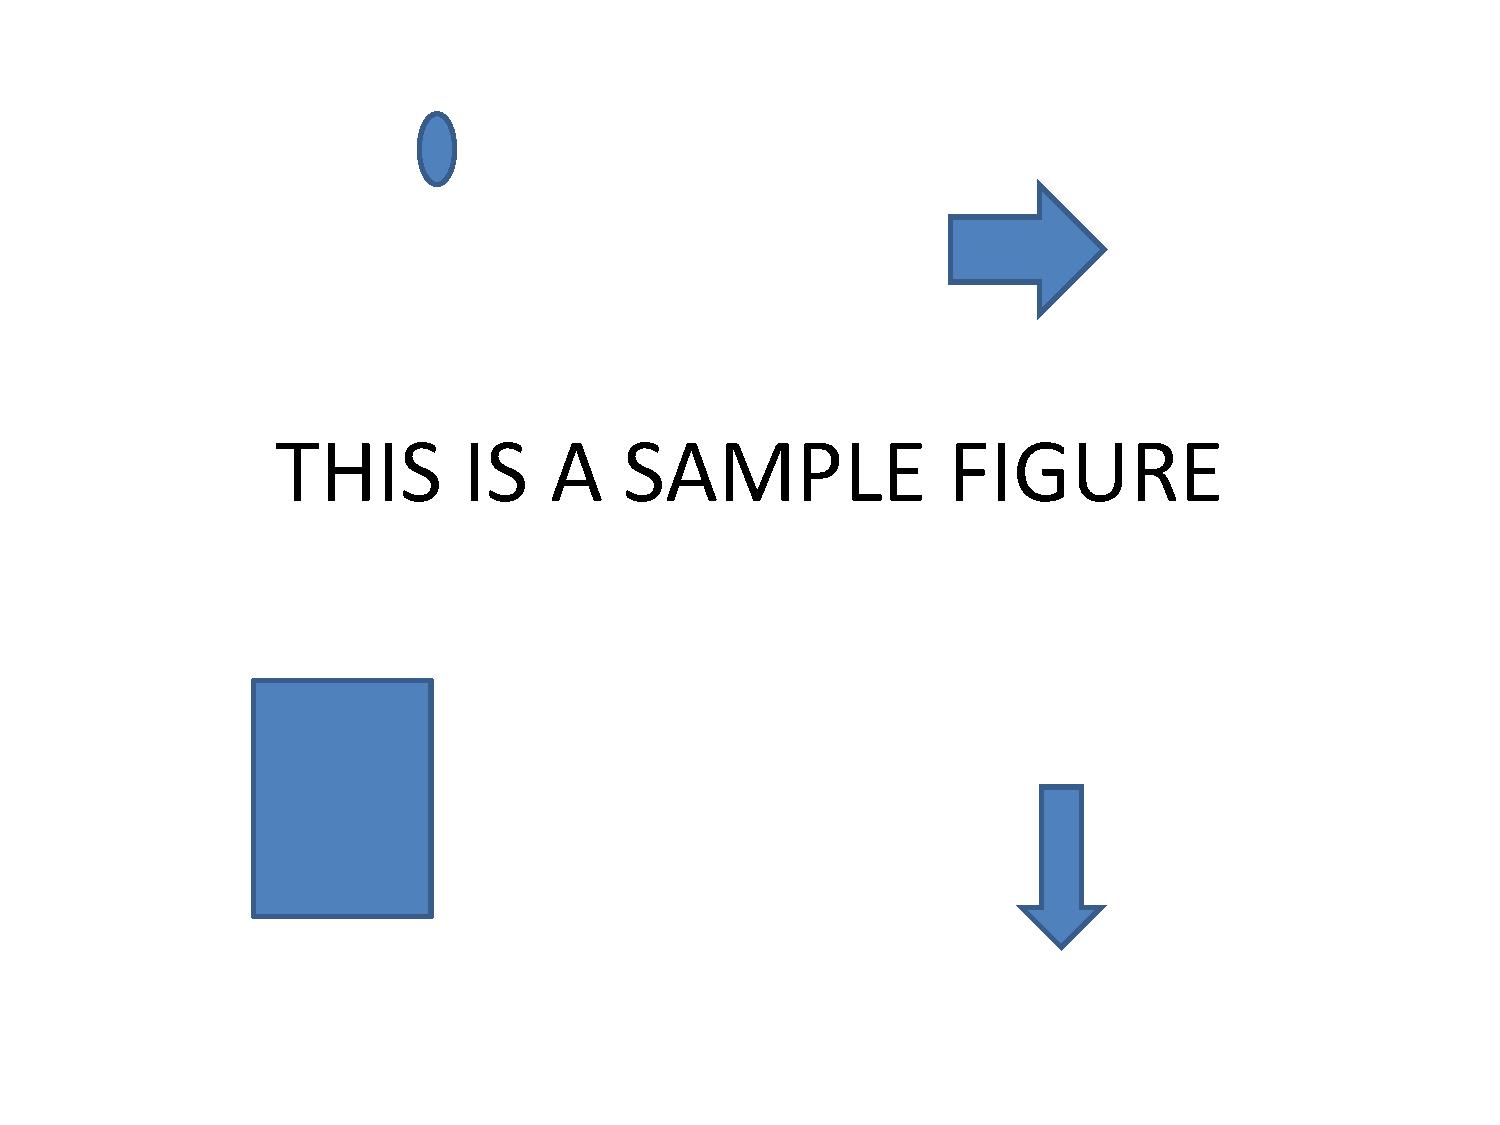
\includegraphics[width=0.5\textwidth,keepaspectratio]{{{Figures/fig1.1_1sample}}}
  \caption[Short caption for TOC.]{This is normal long caption you can write to describe in long figure caption sentence.}\label{fig:fig1.1_1}%
\end{figure}

\section{Research Purpose}\label{ch1:purpose}
Sample research purpose.

\section{Research Outline}\label{ch1:outline}
The remainder of this dissertation is organized as follows.

Chapter~\ref{ch2:sample} focus on how some sample.

Chapter~\ref{ch3:sample} describes about more samples.

Chapter~\ref{ch4:sample} concludes this dissertation.
Finally, limitations of this research and possible research foresights will be briefly explained.

Figure~\ref{fig:1.3_1sample} illustrates the outline of this dissertation.
\begin{figure}[!b]
  \centering%
    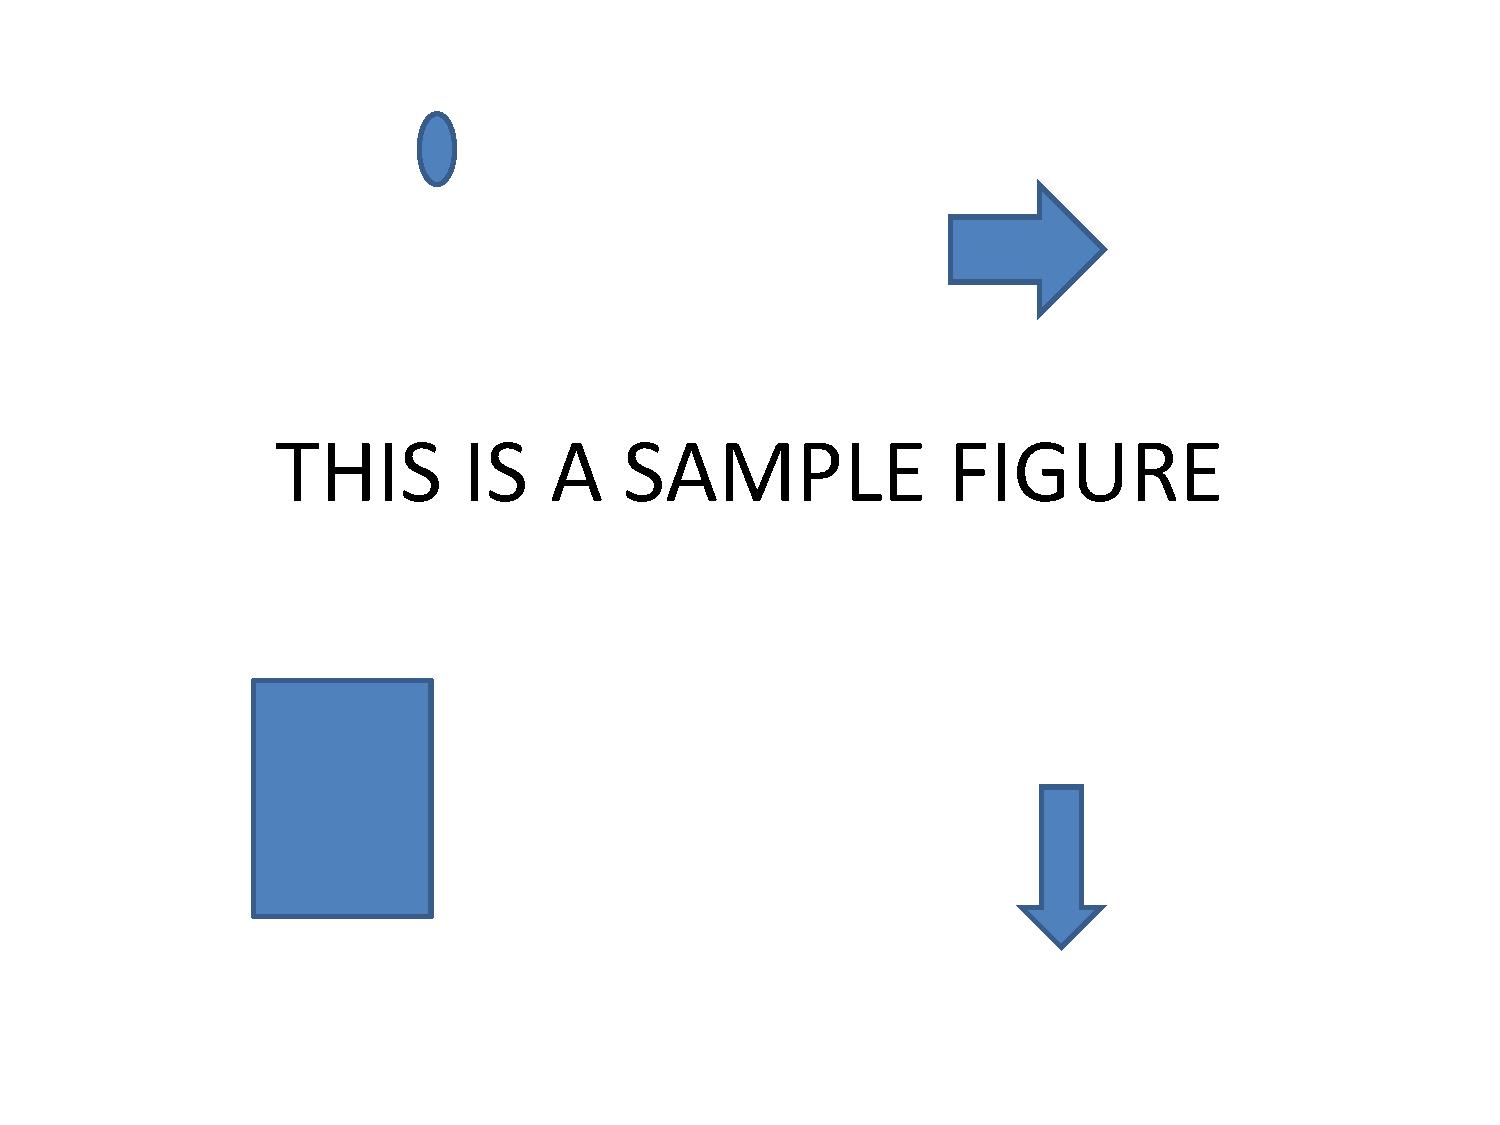
\includegraphics[width=\textwidth,keepaspectratio]{{{Figures/fig1.3_1_to}}}
    \caption{Short caption only one.}\label{fig:1.3_1sample}%
\end{figure}

